\section{Medios de apoyo}

En este apartado se van a definir un conjunto de sistemas que van a ofrecer apoyo en las distintas fases de la implantación del AFUA. Sus funciones se centrarán principalmente en gestionar los espacios aéreos que estarán activos temporalmente. Estos sistemas se encargan de recopilar la información del entorno con el fin de ofrecer las soluciones más óptimas a la hora de asignar los espacios aéreos necesarios para coordinar las operaciones civiles y militares.  

Aunque el principio de funcionamiento de estos sistemas se caracteriza por una gran automatización, será el factor humano el encargado de supervisar y monitorizar todas las acciones que se van a tomar por parte de estos sistemas, interviniendo en caso de que sea necesario.

\subsection{Sistema STANLY / ACOS}

Se trata de una aplicación web para la gestión temporal de espacios aéreos activos temporalmente, ofreciendo apoyo en la fase estratégica, táctica, operacional y posoperatoria.  Es capaz de gestionar áreas como como TRA, VP, áreas peligrosas, áreas restringidas y espacios aéreos prohibidos.  

Este sistema es capaz de calcular la apertura de rutas condicionales basándose en los tiempos de activación de los mismos y los espacios aéreos relacionados. 

\begin{figure}[H]
    \centering
    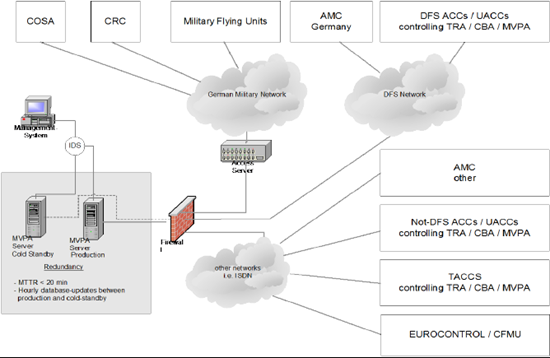
\includegraphics[width=0.8\linewidth]{figuras/stanly_acos.png}
    \caption{Principio de funcionamiento de STANLY / ACOS.}
    \label{fig:stanly_acos}
\end{figure}

Su implantación, también permitirá sustituir las comunicaciones telefónicas de la fase operacional, aunque su coordinación en tiempo real será siempre monitorizada por los agentes correspondientes. 

Se puede acceder a este sistema mediante un buscador web como pude ser Firefox, Chrome o Safari. 

El funcionamiento de este sistema y las relaciones entre los diferentes subsistemas que lo componen se refleja en la figura (\ref{fig:stanly_acos}).

\subsection{Sistema LARA}

El \acrfull{lara} ha sido desarrollado para mejorar la gestión de los procesos relativos a la asignación del espacio aéreo. Para ello se ha basado en proporcionar visibilidad mutua a los requisitos operativos civiles y militares, así como un marco de entendimiento común y habilitando un proceso más eficiente de toma de decisiones colaborativas.
El objetivo es producir un sistema de soporte al ASM armonizado a nivel nacional y regional que permita responder a los requerimientos operacionales de las partes interesadas. El desarrollo de los sistemas LARA está apoyado de manera directa por la Comisión Europea.

LARA es un paquete de software de EUROCONTROL que se ofrece sin cargo adicional a las partes interesadas para apoyar y mejorar los procesos de gestión del espacio aéreo. Ofrece intercambio en tiempo real de los datos relativos a los procesos ASM entre los actores involucrados permitiendo procesos CDM y una mejora de la conciencia situacional de los procesos de gestión.

\begin{figure}[H]
    \centering
    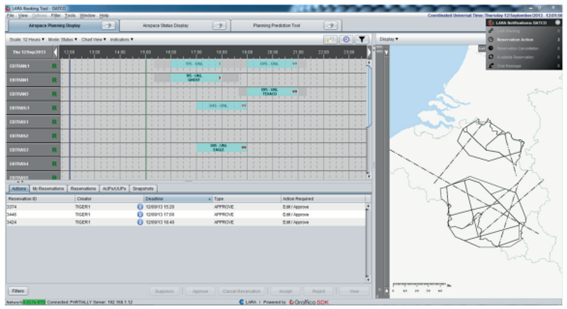
\includegraphics[width=0.8\linewidth]{figuras/lara.png}
    \caption{Pantalla de planificación de LARA.}
    \label{fig:lara}
\end{figure}

La funcionalidad del LARA comprende todas las fases de la gestión del espacio aéreo, desde la planificación en el largo plazo hasta procesos de coordinación en tiempo real.

Además, los sistemas LARA, están capacitados para trabajar interconectados, lo que permite una coordinación entre diferentes Estados y facilitar la eficiencia de las operaciones en zonas fronterizas.

LARA ofrece una interfaz agradable para el usuario que permite la reserva online de espacio aéreo, habilita una coordinación transparente y automatiza las tareas. El sistema está diseñado de manera que se permita configurar todos los parámetros relevantes para adaptarse a los diferentes procesos nacionales, mientras que contribuye a la armonización en la aplicación del concepto de AFUA. 

El aspecto que tiene la pantalla de planificación de espacio aéreo se puede ver en la figura (\ref{fig:lara}).

Además, se indicará si la reserva interfiere con otros espacios aéreos, detectando y resaltando todos los conflictos entre reservas.

Es posible añadir información extra a cada una de las reservas acerca de los detalles de la misión a llevar a cabo. Este tipo de información no es obligatoria, pero puede aportar un valor añadido a la hora realizar estadísticas y mejorar la coordinación de los procesos entre los diferentes actores. Por razones de confidencialidad, estos detalles únicamente estarán disponibles para aquellos usuarios autorizados.

\begin{figure}[H]
    \centering
    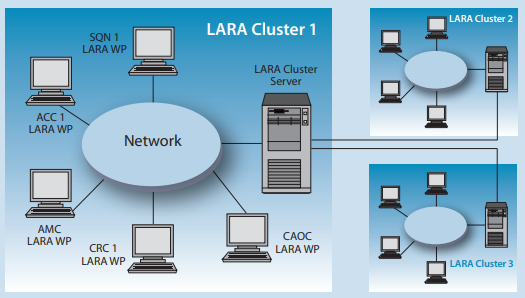
\includegraphics[width=0.8\linewidth]{figuras/lara_cluster.png}
    \caption{Conexión de \textit{clusters} de LARA.}
    \label{fig:lara_cluster}
\end{figure}

El sistema LARA está organizado en grupos (clusters), que normalmente están definidos por las fronteras nacionales, pero que pueden ser adaptados a cualquier tipo de organización, como podrían ser los bloques funcionales de espacio aéreo (FAB). Cada grupo gestiona un servidor central al que están conectados los diferentes clientes.

Los diferentes \textit{clusters} pueden estar interconectados como se muestra en la figura (\ref{fig:lara_cluster}).



\subsection{Sistema iADS}

iADS es una herramienta de gestión del espacio aéreo diseñada para mejorar la colaboración en la toma de decisiones entre los organismos civiles y militares en la gestión de la red local. iADS muestra gráficamente la demanda de espacio aéreo y, teniendo en cuenta las limitaciones pertinentes, como los niveles de personal, las configuraciones de los sectores, los valores de los monitores de los sectores y los datos meteorológicos pertinentes, la capacidad del espacio aéreo. iADs proporciona una pantalla visual fácilmente interpretable que permite a los organismos de gestión de la red local comprender plenamente el impacto de las decisiones de asignación del espacio aéreo y proporciona la capacidad de ajustar la asignación del espacio aéreo con el fin de hacer el mejor uso del espacio aéreo disponible.

El conocimiento mutuo de la demanda de espacio aéreo y de los factores que afectan a la demanda, así como una función gráfica "what if" para simular cambios en las reservas solicitadas y en las rutas de las aeronaves, mejora la coordinación y permite optimizar la capacidad del espacio aéreo en beneficio de los usuarios del espacio aéreo civil y militar a nivel local, además de contribuir a la optimización a nivel de red. Este concepto se puede ver en la figura (\ref{fig:iads}).

\begin{figure}[H]
    \centering
    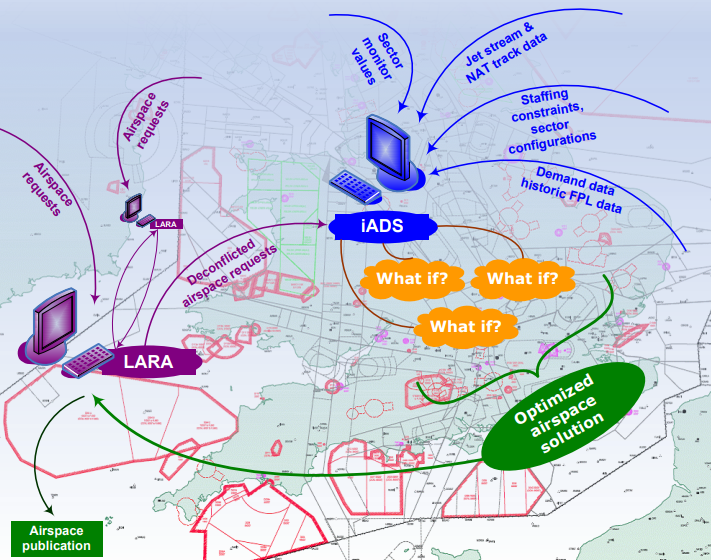
\includegraphics[width=0.6\linewidth]{figuras/iads.png}
    \caption{Concepto iADS.}
    \label{fig:iads}
\end{figure}

iADS se provee mediante un servidor basado en Microsoft (MS) Windows que aloja una base de datos SQL y la aplicación iADS. El servicio está basado en la web y se proporciona a través de una red basada en IP a clientes basados en Windows, utilizando MS Internet Explorer y MS Silverlight. La entrada de datos del sistema en el prototipo se realiza actualmente mediante la transferencia manual de archivos. La entrada de datos manual se realiza mediante la interacción con el cliente. En la figura (\ref{fig:iads_map}) se puede observar la interfaz del programa, donde aparece en el mapa la información relevante.

El sistema iADS se utiliza para las distintas fases de planificación. La fase 1 de iADS es el inicio de un desarrollo escalonado que apoya los procesos y procedimientos actuales dentro de la toma de decisiones en colaboración con el ASM y el ATFCM. La fase 1 se centra en la toma de decisiones dentro de la escala temporal D-7 a D-3; la fase 2 se centra en la introducción de la toma de decisiones automatizada y controlada por parámetros, y en la optimización del espacio aéreo en el periodo D-3 a D-1; la fase 3 lleva estas mejoras al día de las operaciones. 

El iADS muestra las solicitudes de reserva de espacio aéreo militar, los flujos de tráfico civil y las cargas de los sectores codificadas por colores para poner de manifiesto los desequilibrios de la demanda y la capacidad. iADS permite a los organismos de gestión de la red local plantear escenarios de asignación del espacio aéreo mediante la limitación de niveles o el desplazamiento (tanto geográfico como temporal) de las solicitudes de espacio aéreo, el desvío del tráfico civil y el encasillamiento o la división de los sectores ATC. Esta característica se puede observar en la figura (\ref{fig:iads_request}), donde aparecen las peticiones de espacio aéreo de los distintos usuarios.

\begin{figure}[H]
    \centering
    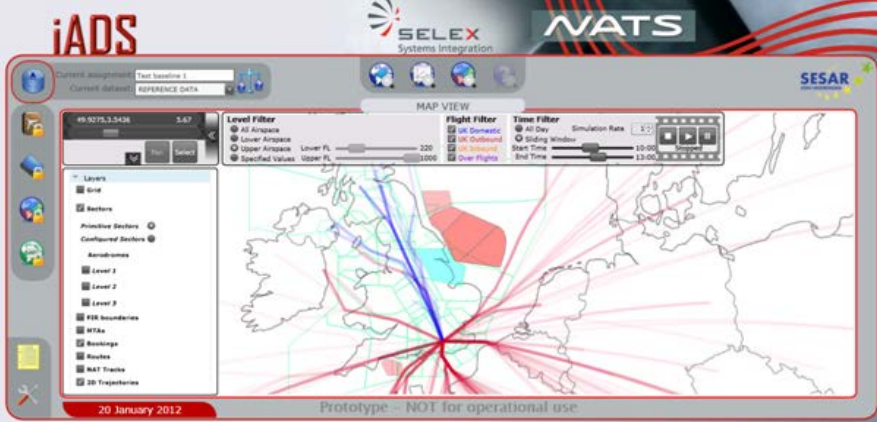
\includegraphics[width=1\linewidth]{figuras/iads_map.png}
    \caption{Vista del mapa en iADS.}
    \label{fig:iads_map}
\end{figure}

\begin{figure}[H]
    \centering
    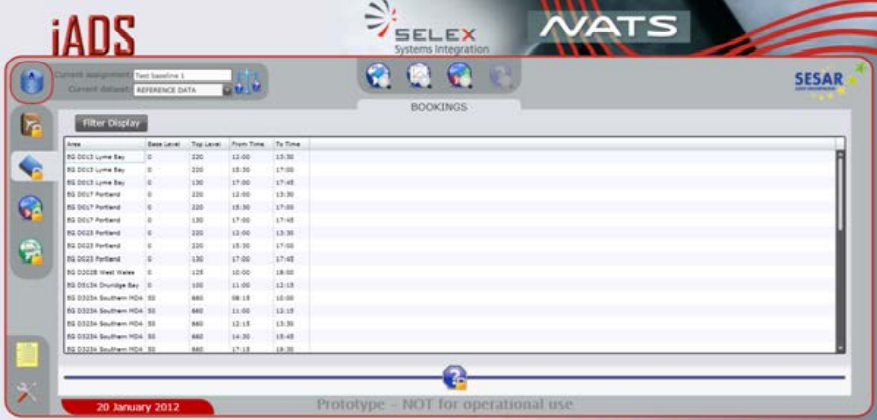
\includegraphics[width=1\linewidth]{figuras/iads_request.png}
    \caption{Peticiones de espacio aéreo en iADS.}
    \label{fig:iads_request}
\end{figure}